\MathBookSourcePage{109}
\appendix
\chapter{标准有限元逼近的结果}\label{app:standard-finite-element-approximation}
\counterwithout{equation}{section}
\renewcommand{\theequation}{A.\arabic{equation}}
\renewcommand{\thestatement}{A.\arabic{statement}}
\renewcommand{\thefigure}{\arabic{figure}}
\setcounter{equation}{0}
\setcounter{statement}{0}
\setcounter{figure}{2}

本附录汇集了后文将用到的经典有限元逼近的大部分性质.
较为熟悉的结果将不加证明地陈述; 关于详细证明和进一步材料,
读者可参阅 Ciarlet [19] 以及 Strang \& Fix [77] 的内容完备的著作.
此外, 我们还简要提及一些较新或非标准的材料,
其中包括 Clément [21], Bernardi [9], Scott [73] 和 Lenoir [50]
等人发展的结果, 它们在后文中也会十分有用.

\section{三角形有限元}\label{sec:appendix-triangular-finite-elements}

\begin{Definition}\label{def:appendix-polynomial-space-pk}
对每个整数 $k\geq0$, 记 $P_k$ 为 $\mathbb{R}^N$ 上次数不超过 $k$
的所有多项式构成的空间.
\end{Definition}

回顾一下, $\mathbb{R}^N$ 中的一个 $N$-单形是 $N+1$ 个点
$a_j$, $1\leq j\leq N+1$, 的凸包 $\kappa$, 这些点称为
$\kappa$ 的顶点, 并且它们不全位于同一个超平面内.
例如, $2$-单形是非退化三角形, $3$-单形是非退化四面体.
一个 $N$-单形 $\kappa$ 的大小和形状由两个量描述:
\[
h_\kappa=\text{$\kappa$ 的直径}
\]
以及
\[
\rho_\kappa
=
\sup\{\,\text{$B$ 的直径};\ \text{$B$ 是包含于 $\kappa$ 中的球}\,\}.
\]
此外, $\kappa$ 的正则性由比值
\[
\sigma_\kappa=h_\kappa/\rho_\kappa
\]
度量.

在参考空间 $(\hat x_1,\ldots,\hat x_N)$ 中, 记参考单位单形为
$\hat\kappa$, 其顶点为
$\hat a_j=(\delta_{ij})_{1\leq i\leq N}$, $1\leq j\leq N$,
以及 $\hat a_{N+1}=(0)_{1\leq i\leq N}$.
若 $\kappa$ 是顶点为 $a_j$, $1\leq j\leq N+1$, 的 $N$-单形,
则恰有一个仿射映射
\begin{equation}\label{eq:appendix-simplex-affine-map}
F_\kappa(\hat x)=B_\kappa\hat x+b_\kappa
\end{equation}
把 $\hat\kappa$ 映到 $\kappa$, 并满足
$F_\kappa(\hat a_i)=a_i$, $1\leq i\leq N+1$.
由此容易证明矩阵 $B_\kappa$ 非奇异, 且满足
\begin{equation}\label{eq:appendix-simplex-matrix-bounds}
\|B_\kappa\|\leq h_\kappa/\rho_{\hat\kappa},
\qquad
\|B_\kappa^{-1}\|\leq h_{\hat\kappa}/\rho_\kappa,
\end{equation}
其中 $\|\cdot\|$ 同时表示 $\mathbb{R}^N$ 的 Euclidean 范数及其从属矩阵范数.
此外, 由于
\begin{equation}\label{eq:appendix-simplex-determinant-measure}
|\det(B_\kappa)|
=
\operatorname{meas}(\kappa)/\operatorname{meas}(\hat\kappa),
\end{equation}
存在仅依赖于 $N$ 的两个正常数 $C_1(N)$ 和 $C_2(N)$, 使得
\begin{equation}\label{eq:appendix-simplex-determinant-bounds}
C_2(N)\rho_\kappa^N
\leq
|\det(B_\kappa)|
\leq
C_1(N)h_\kappa^N.
\end{equation}

为了方便, 有时将 $\mathbb{R}^N$ 中一点 $x$ 的 Euclidean 坐标换成
它关于顶点 $a_i$, $1\leq i\leq N+1$, 的重心坐标
$\lambda_i=\lambda_i(x)$, 其定义为
\begin{equation}\label{eq:appendix-barycentric-coordinate-definition}
\lambda_i\in P_1,
\qquad
\lambda_i(a_j)=\delta_{ij},
\qquad
1\leq i,j\leq N+1.
\end{equation}
重心坐标在 $\mathbb{R}^N$ 中满足下列有用的恒等式:
\begin{equation}\label{eq:appendix-barycentric-identities}
\sum_{i=1}^{N+1}\lambda_i=1,
\qquad
p=\sum_{i=1}^{N+1}p(a_i)\lambda_i
\quad
\forall p\in P_1.
\end{equation}
此外, 容易验证
\[
\kappa
=
\{\,x\in\mathbb{R}^N;\ 0\leq\lambda_i(x)\leq1,
\ 1\leq i\leq N+1\,\}.
\]

\begin{figure}[htbp]
\centering
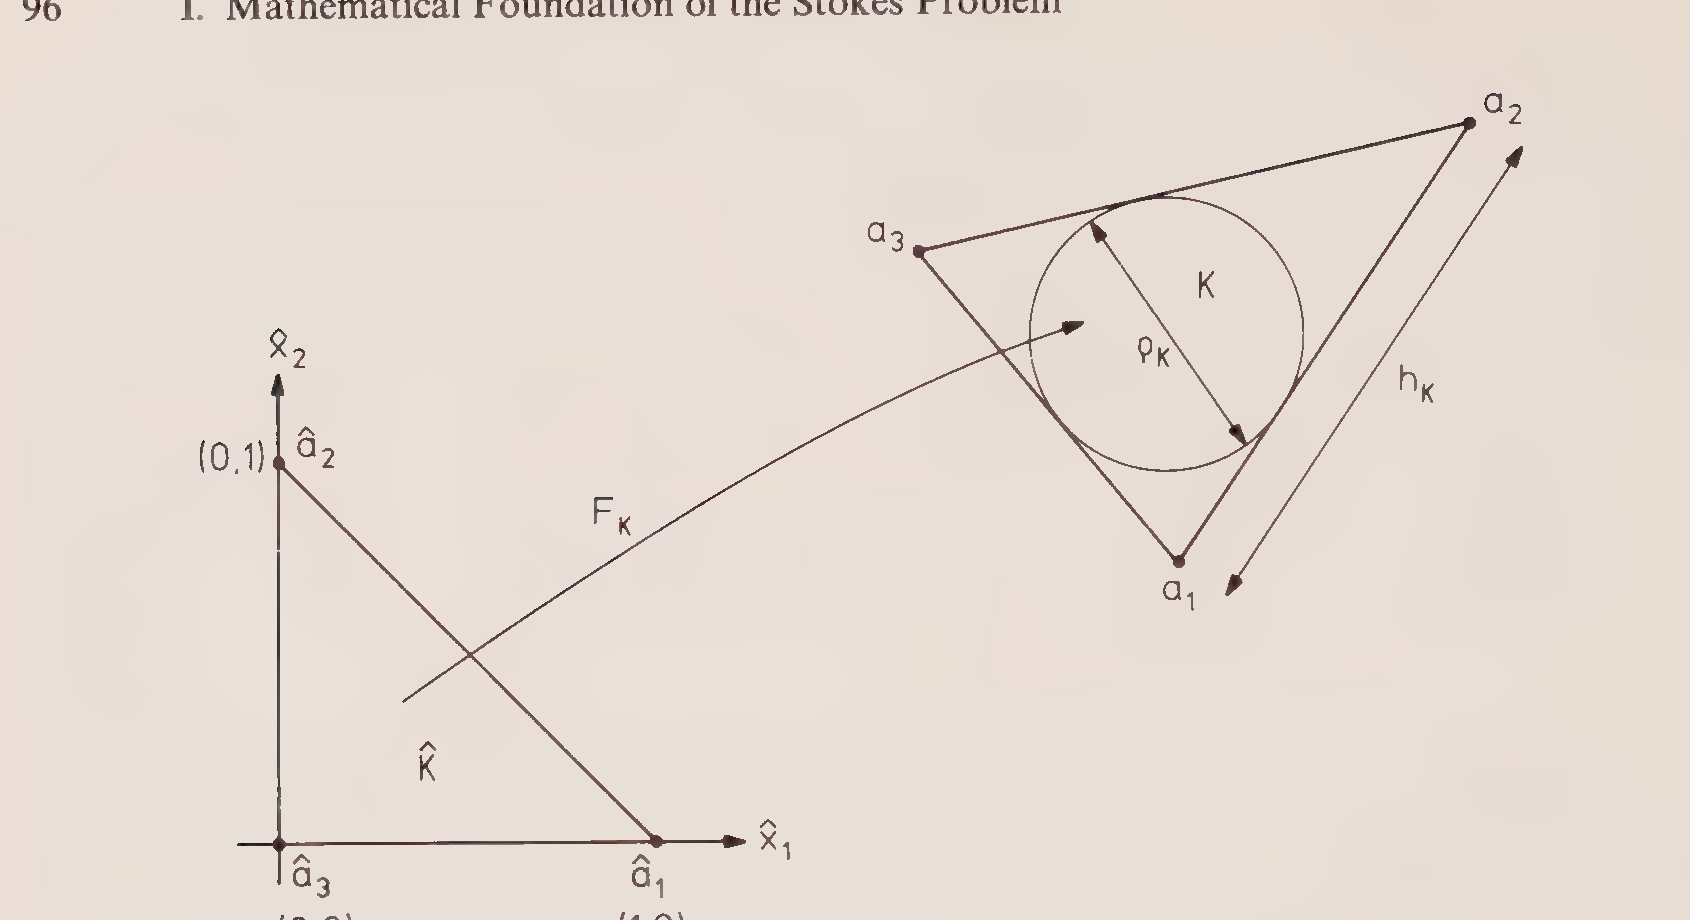
\includegraphics[width=.88\linewidth]{figures/appendix-figure-3.png}
\caption{三角形 $\kappa$ 及其参考单位三角形 $\hat\kappa$ ($N=2$).}
\label{fig:appendix-triangle-reference-simplex}
\end{figure}

如前所述, 映射 $x=F_\kappa(\hat x)$ 在 $\hat\kappa$ 与 $\kappa$
之间建立一一对应. 与 $F_\kappa$ 以及 $F_\kappa^{-1}$ 的复合
\[
(v:\kappa\to\mathbb{R})
\longmapsto
(\hat v=v\circ F_\kappa:\hat\kappa\to\mathbb{R})
\]
和
\[
(\hat v:\hat\kappa\to\mathbb{R})
\longmapsto
(v=\hat v\circ F_\kappa^{-1}:\kappa\to\mathbb{R})
\]
会经常使用, 因为它们使我们能够只在参考单元 $\hat\kappa$ 上工作.
这种变量变换的影响由下面的 Lemma 给出.

\setcounter{statement}{0}
\begin{Lemma}\label{lem:appendix-simplex-change-of-variables}
对每个整数 $m\geq0$ 以及每个满足 $1\leq p\leq\infty$ 的实数 $p$,
映射 $v\mapsto\hat v=v\circ F_\kappa$ 是从 $W^{m,p}(\kappa)$
到 $W^{m,p}(\hat\kappa)$ 的同构, 并且有下列估计:
\begin{align}
|\hat v|_{m,p,\hat\kappa}
&\leq
C_1\|B_\kappa\|^m
|\det(B_\kappa)|^{-1/p}|v|_{m,p,\kappa}
&&\forall v\in W^{m,p}(\kappa),
\label{eq:appendix-change-forward}\\
|v|_{m,p,\kappa}
&\leq
C_2\|B_\kappa^{-1}\|^m
|\det(B_\kappa)|^{1/p}|\hat v|_{m,p,\hat\kappa}
&&\forall\hat v\in W^{m,p}(\hat\kappa).
\label{eq:appendix-change-inverse}
\end{align}
\end{Lemma}

注意, 函数的梯度和单位法向量具有简单的表达式
(例如参见 Babuška \& Aziz [5]):
\begin{align}
\operatorname{grad}_{\hat x}\hat v(\hat x)
&=
(B_\kappa^T\operatorname{grad}_x v)\circ F_\kappa(\hat x),
\label{eq:appendix-gradient-transform}\\
\hat{\mathbf n}(\hat x)
&=
\left[
\frac{B_\kappa^T\mathbf n}{\|B_\kappa^T\mathbf n\|}
\right]\circ F_\kappa(\hat x),
\label{eq:appendix-normal-transform}
\end{align}
其中 $\mathbf n$(相应地, $\hat{\mathbf n}$) 表示 $\kappa$(相应地,
$\hat\kappa$) 的单位外法向量.

下面的 Theorem 是 Theorem \ref{thm:peetre-tartar-compact-operator}
的一个推广, 它及其推论是有限元理论的基本工具.

\setcounter{statement}{0}
\begin{Theorem}\label{thm:appendix-bramble-hilbert-general}
对每个整数 $k\geq0$ 以及满足 $1\leq p\leq\infty$ 的实数 $p$,
存在一个仅依赖于 $k$, $p$ 和 $\hat\kappa$ 的常数 $\hat C>0$, 使得
\begin{equation}\label{eq:appendix-bramble-hilbert}
\inf_{t\in P_k}
\|\hat u+t\|_{k+1,p,\hat\kappa}
\leq
\hat C|\hat u|_{k+1,p,\hat\kappa}
\qquad
\forall\hat u\in W^{k+1,p}(\hat\kappa)/P_k.
\end{equation}
\end{Theorem}

\setcounter{statement}{0}
\begin{Corollary}\label{cor:appendix-abstract-interpolation-reference}
设 $k\geq0$, $m\geq0$ 为整数, $p\geq1$, $q\geq1$ 为实数, 且
\[
W^{k+1,p}(\hat\kappa)\hookrightarrow W^{m,q}(\hat\kappa).
\]
设
$\hat\pi\in\mathcal{L}(W^{k+1,p}(\hat\kappa);W^{m,q}(\hat\kappa))$
满足
\[
\hat\pi t=t
\qquad
\forall t\in P_k.
\]
则存在一个仅依赖于 $k$, $m$, $p$, $q$, $\hat\kappa$ 和 $\hat\pi$
的常数 $\hat C>0$, 使得
\begin{equation}\label{eq:appendix-abstract-interpolation-reference}
\|\hat v-\hat\pi\hat v\|_{m,q,\hat\kappa}
\leq
\hat C|\hat v|_{k+1,p,\hat\kappa}
\qquad
\forall\hat v\in W^{k+1,p}(\hat\kappa).
\end{equation}
\end{Corollary}

将 Lemma \ref{lem:appendix-simplex-change-of-variables},
\eqref{eq:appendix-simplex-matrix-bounds} 和
\eqref{eq:appendix-simplex-determinant-measure}
与 Corollary \ref{cor:appendix-abstract-interpolation-reference} 结合, 得到:

\setcounter{statement}{1}
\begin{Corollary}\label{cor:appendix-abstract-interpolation-physical}
设 $k$, $m$, $p$, $q$ 和 $\hat\pi$ 如 Corollary
\ref{cor:appendix-abstract-interpolation-reference} 中所述.
设 $\kappa$ 是 $\mathbb{R}^N$ 中的一个 $N$-单形, 并定义
$\pi\in\mathcal{L}(W^{k+1,p}(\kappa);W^{m,q}(\kappa))$ 为
\begin{equation}\label{eq:appendix-interpolant-commuting-definition}
(\pi v)\circ F_\kappa
=
\hat\pi(v\circ F_\kappa)
\quad
(\text{即 }\widehat{\pi v}=\hat\pi\hat v).
\end{equation}
则存在一个仅依赖于 $k$, $m$, $p$, $q$, $\hat\kappa$ 和 $\hat\pi$
的常数 $C>0$, 使得对所有 $v\in W^{k+1,p}(\kappa)$ 有
\begin{equation}\label{eq:appendix-abstract-interpolation-physical}
|v-\pi v|_{m,q,\kappa}
\leq
C\sigma_\kappa^m
(\operatorname{meas}(\kappa))^{1/q-1/p}
h_\kappa^{k+1-m}
|v|_{k+1,p,\kappa}.
\end{equation}
\end{Corollary}

\MathBookSourcePage{112}
从现在起, 除了某些会在 $N$ 维情形中陈述的结果之外,
我们假定维数 $N$ 等于 $2$.
此外, 为简化讨论, 假设 $\Omega$ 是边界 $\Gamma$ 为多边形的有界区域.
曲边所固有的技术困难可以利用 Bernardi [9] 引入的一般单元方便地处理,
但这里没有篇幅讨论它们.

对每个 $h>0$, 设 $\mathcal{T}_h$ 是 $\bar\Omega$ 的一个三角剖分,
它由直径不超过 $h$ 的闭三角形 $\kappa$ 组成. 换言之,
\[
\bar\Omega
=
\bigcup_{\kappa\in\mathcal{T}_h}\kappa,
\qquad
h_\kappa\leq h,
\]
且任意两个三角形要么不相交, 要么恰好共用一条边或一个顶点.

\setcounter{statement}{1}
\begin{Definition}\label{def:appendix-regular-triangulation}
$1^\circ)$ 若存在与 $h$ 和 $\kappa$ 无关的数 $\sigma>0$, 使得当
$h\to0$ 时
\begin{equation}\label{eq:appendix-regular-triangulation}
\sigma_\kappa\leq\sigma
\qquad
\forall\kappa\in\mathcal{T}_h,
\end{equation}
则称三角剖分族 $\mathcal{T}_h$ 是正则的.

$2^\circ)$ 此外, 若存在另一个常数 $\tau>0$, 使得当 $h\to0$ 时
\begin{equation}\label{eq:appendix-uniformly-regular-triangulation}
\tau h\leq h_\kappa\leq\sigma\rho_\kappa
\qquad
\forall\kappa\in\mathcal{T}_h,
\end{equation}
则称 $\mathcal{T}_h$ 是一致正则的(或拟一致的).
\end{Definition}

\setcounter{statement}{0}
\begin{Remark}\label{rem:appendix-local-interpolation-estimate}
当 $\mathcal{T}_h$ 正则时, 误差估计
\eqref{eq:appendix-abstract-interpolation-physical} 简化为
\begin{equation}\label{eq:appendix-local-interpolation-estimate}
|v-\pi v|_{m,q,\kappa}
\leq
Ch_\kappa^{k+1-m+N(1/q-1/p)}
|v|_{k+1,p,\kappa}
\qquad
\forall v\in W^{k+1,p}(\kappa),
\end{equation}
其中常数 $C$ 与 $v$, $h$ 和 $\kappa$ 无关.
由于嵌入
$W^{k+1,p}(\hat\kappa)\hookrightarrow W^{m,q}(\hat\kappa)$,
有
\[
k+1-m+N(1/q-1/p)\geq0,
\]
因此上式中的因子 $h_\kappa$ 可以由 $h$ 控制.
\end{Remark}

现在固定整数 $k\geq1$, 并引入标准有限元空间
\begin{equation}\label{eq:appendix-standard-triangular-fem-spaces}
\begin{aligned}
\Theta_h
&=
\{\,\theta_h\in\mathcal{C}^0(\bar\Omega);
\ \theta_h|_\kappa\in P_k
\quad\forall\kappa\in\mathcal{T}_h\,\},\\
\Phi_h
&=
\Theta_h\cap H_0^1(\Omega).
\end{aligned}
\end{equation}
注意, 它们都是 $W^{1,\infty}(\Omega)$ 的有限维子空间,
但当逼近参数 $h\to0$ 时, 它们的维数趋于无穷.

接着定义插值算子. 最简单的选择是在 $N$-单形 $\kappa$
的一组适当点上插值函数, 例如 $k$ 阶主格点
\begin{equation}\label{eq:appendix-principal-lattice-simplex}
\Sigma_\kappa
=
\left\{\,
x=\sum_{j=1}^{N+1}\lambda_ja_j;
\ \sum_{j=1}^{N+1}\lambda_j=1,
\ \lambda_j\in\{0,1/k,\ldots,(k-1)/k,1\},
\ 1\leq j\leq N+1
\,\right\}.
\end{equation}
参见 Figure \ref{fig:appendix-principal-lattice-order-three} 中 $k=3$ 的情形.

\begin{figure}[htbp]
\centering
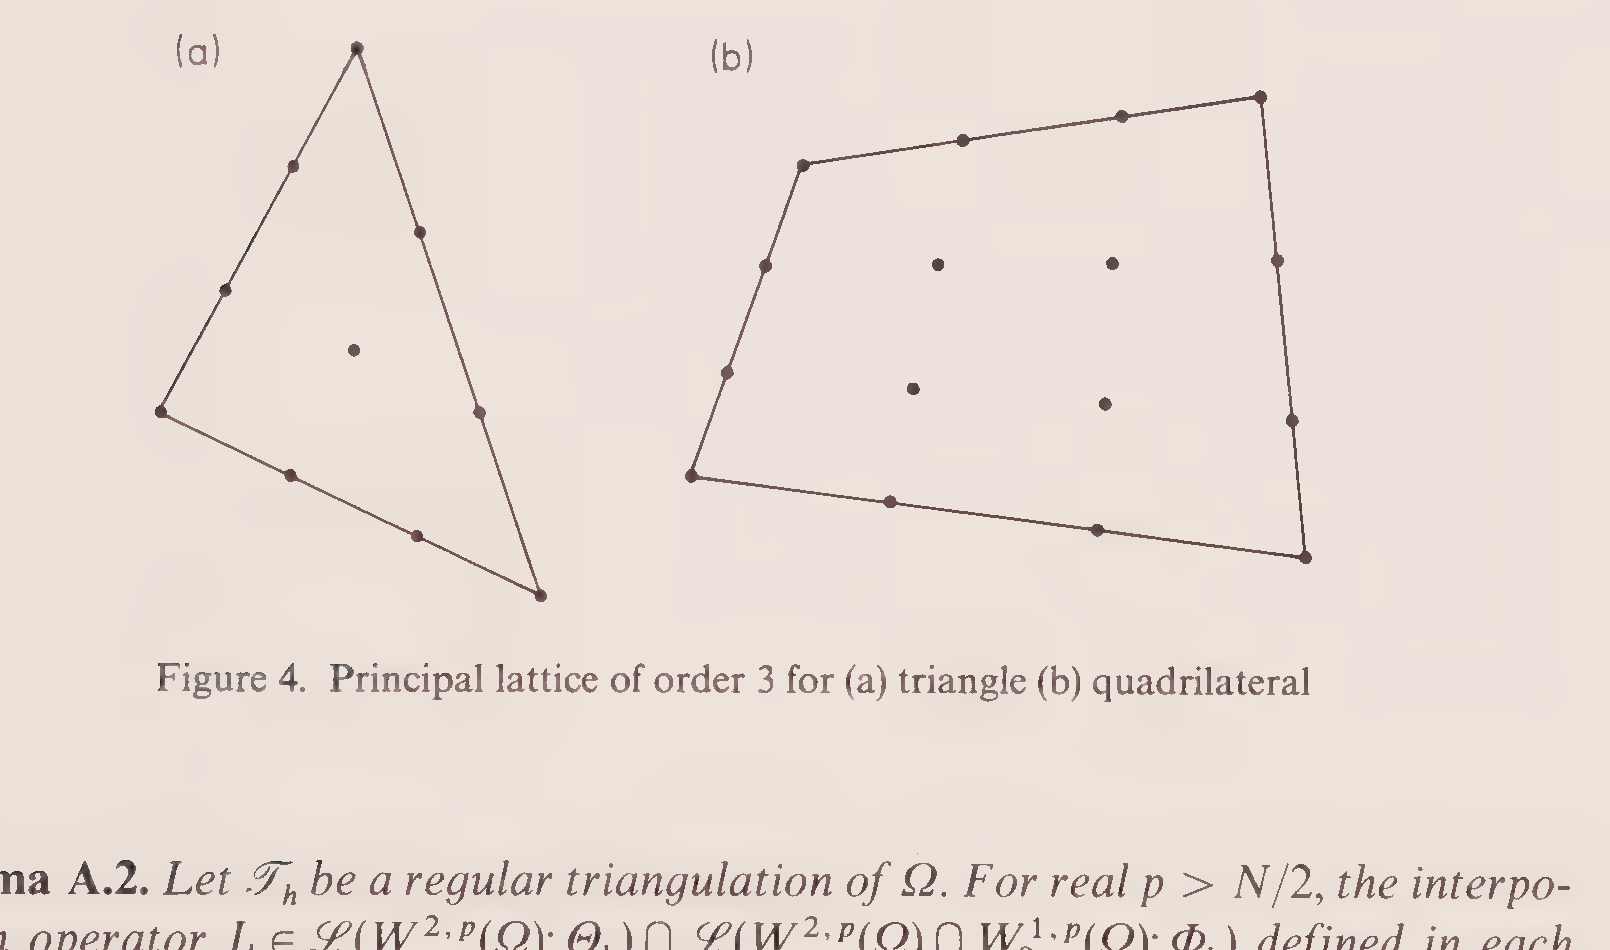
\includegraphics[width=.82\linewidth]{figures/appendix-figure-4.png}
\caption{$3$ 阶主格点: (a) 三角形; (b) 四边形.}
\label{fig:appendix-principal-lattice-order-three}
\end{figure}

由此得到一个广泛使用并具有众所周知性质的插值算子 $I_h$,
这些性质在所有维数 $N$ 中都成立.

\setcounter{statement}{1}
\begin{Lemma}\label{lem:appendix-lagrange-interpolation}
设 $\mathcal{T}_h$ 是 $\Omega$ 的一个正则三角剖分.
对实数 $p>N/2$, 在每个单元 $\kappa$ 上由
\begin{equation}\label{eq:appendix-lagrange-interpolant-definition}
I_hv|_\kappa\in P_k,
\qquad
I_hv(x)=v(x)
\quad
\forall x\in\Sigma_\kappa
\end{equation}
定义的插值算子
\[
I_h\in\mathcal{L}(W^{2,p}(\Omega);\Theta_h)
\cap
\mathcal{L}(W^{2,p}(\Omega)\cap W_0^{1,p}(\Omega);\Phi_h)
\]
对所有满足 $0\leq m\leq s+1$, $1\leq s\leq k$ 的整数 $m$
和实数 $s$ 有误差估计
\begin{subequations}
\begin{equation}\label{eq:appendix-lagrange-interpolation-error-wsp}
|v-I_hv|_{m,p,\Omega}
\leq
C_1h^{s+1-m}|v|_{s+1,p,\Omega}
\qquad
\forall v\in W^{s+1,p}(\Omega).
\end{equation}
此外, 对所有实数 $q>N$,
\[
I_h\in\mathcal{L}(W^{1,q}(\Omega);\Theta_h)
\cap
\mathcal{L}(W_0^{1,q}(\Omega);\Phi_h),
\]
并且
\begin{equation}\label{eq:appendix-lagrange-interpolation-error-w1q}
|v-I_hv|_{m,q,\Omega}
\leq
C_2h^{1-m}|v|_{1,q,\Omega}
\qquad
\forall v\in W^{1,q}(\Omega),
\quad m=0,1.
\end{equation}
\end{subequations}
两个常数 $C_1$ 和 $C_2$ 都为正, 且与 $h$ 和 $v$ 无关.
\end{Lemma}

然而, 在后续应用中, 使用一个略有不同的插值算子有时更为方便.
下面在 $N=2$ 时给出它.
